%!TEX TS-program = pdflatex
%!TEX encoding = utf8
\documentclass[12pt, oneside]{book}
\usepackage[T1]{fontenc}
\usepackage[utf8]{inputenc}
\usepackage[english]{babel}
%% FONTS: libertine+biolinum+stix
\usepackage[mono=false]{libertine}
\usepackage[backend=biber, style=nature, citestyle=numeric, sorting=none]{biblatex}
\addbibresource{references.bib}

\usepackage{graphicx}
\usepackage{caption}
\usepackage{subcaption}

% =====================
% = Datos importantes =
% =====================
% hay que rellenar estos datos y luego
% ir a \begin{document}

\title{Simulation and implementation of a Conformal Finite Difference Time Domain method}
\author{Carlos Julio Ramos Salas}
\date{30 Junio 2024}
\newcommand{\tutores}[1]{\newcommand{\guardatutores}{#1}}
\tutores{Dr. Luis Manuel Díaz Angulo \\
         Dr. Kenan Tekbaş}

% ======================
% = Páginas de títulos =
% ======================
\makeatletter
\edef\maintitle{\@title}
\renewcommand\maketitle{%
  \begin{titlepage}
      \vspace*{1.5cm}
      \parskip=0pt
      \Huge\bfseries
      \begin{center}
          \leavevmode
\includegraphics[totalheight=6cm]{Imagenes/sello.jpg}\\[2cm]
          \@title
      \end{center}
      \vspace{1cm}
      \begin{center}
          \@author
      \end{center}
  \end{titlepage}
  
  \begin{titlepage}
  \parindent=0pt
  \begin{flushleft}
  \vspace*{1.5mm}
  \setlength\baselineskip{0pt}
  \setlength\parskip{0mm}
  \begin{center}
      \leavevmode
\includegraphics[totalheight=4.5cm]{Imagenes/sello.jpg}
  \end{center}
  \end{flushleft}
  \vspace{1cm}
  \bgroup
  \Large \bfseries
  \begin{center}
  \@title
  \end{center}
  \egroup
  \vspace*{.5cm}
  \begin{center}
  \@author
  \end{center}
  \vspace*{1.8cm}
  \begin{flushright}
  \begin{minipage}{8.45cm}
      Memoria del {\bf Trabajo Fin de Máster}.\\ 
      Máster en Física y Matemáticas (FisyMat) \\ 
      University of Granada (UGR).

      \vspace*{7.5mm}

      Tutored by:
      % \vspace*{5mm}
  \end{minipage}\par
  \begin{tabularx}{8.45cm}[b]{@{}l}
      \guardatutores
  \end{tabularx}
   \end{flushright}
      \vspace*{\fill}
   \end{titlepage}
   %%% Esto es necesario...
   \pagestyle{tfg}
   \renewcommand{\chaptermark}[1]{\markright{\thechapter.\space ##1}}
   \renewcommand{\sectionmark}[1]{}
   \renewcommand{\subsectionmark}[1]{}
  }
\makeatother

% ======================================
% = Color de la Universidad de Sevilla =
% ======================================
\usepackage{tikz}
\definecolor{USred}{cmyk}{0,1.00,0.65,0.34}

% =========
% = Otros =
% =========
\usepackage[]{tabularx}
\usepackage[]{enumitem}
\setlist{noitemsep}

% ==========================
% = Matemáticas y teoremas =
% ==========================
\usepackage[]{amsmath}
\usepackage[]{amsthm}
\usepackage[]{mathtools}
\usepackage[]{bm}
\usepackage[]{thmtools}
\newcommand{\marcador}{\vrule height 10pt depth 2pt width 2pt \hskip .5em\relax}
\newcommand{\cabeceraespecial}{%
    \color{USred}%
    \normalfont\bfseries}
\declaretheoremstyle[
    spaceabove=\medskipamount,
    spacebelow=\medskipamount,
    headfont=\cabeceraespecial\marcador,
    notefont=\cabeceraespecial,
    notebraces={(}{)},
    bodyfont=\normalfont\itshape,
    postheadspace=1em,
    numberwithin=chapter,
    headindent=0pt,
    headpunct={.}
    ]{importante}
\declaretheoremstyle[
    spaceabove=\medskipamount,
    spacebelow=\medskipamount,
    headfont=\normalfont\itshape\color{USred},
    notefont=\normalfont,
    notebraces={(}{)},
    bodyfont=\normalfont,
    postheadspace=1em,
    numberwithin=chapter,
    headindent=0pt,
    headpunct={.}
    ]{normal}
\declaretheoremstyle[
    spaceabove=\medskipamount,
    spacebelow=\medskipamount,
    headfont=\normalfont\itshape\color{USred},
    notefont=\normalfont,
    notebraces={(}{)},
    bodyfont=\normalfont,
    postheadspace=1em,
    headindent=0pt,
    headpunct={.},
    numbered=no,
    qed=\color{USred}\marcador
    ]{demostracion}

% Los nombres de los enunciados. Añade los que necesites.
\declaretheorem[name=Observaci\'on, style=normal]{remark}
\declaretheorem[name=Corolario, style=normal]{corollary}
\declaretheorem[name=Proposici\'on, style=normal]{proposition}
\declaretheorem[name=Lema, style=normal]{lemma}

\declaretheorem[name=Teorema, style=importante]{theorem}
\declaretheorem[name=Definici\'on, style=importante]{definition}

\let\proof=\undefined
\declaretheorem[name=Demostraci\'on, style=demostracion]{proof}


% ============================
% = Composición de la página =
% ============================
\usepackage[
    a4paper,
    textwidth=80ex,
]{geometry}

\linespread{1.069}
\parskip=10pt plus 1pt minus .5pt
\frenchspacing
% \raggedright


% ==============================
% = Composición de los títulos =
% ==============================

\usepackage[explicit]{titlesec}

\newcommand{\hsp}{\hspace{20pt}}
\titleformat{\chapter}[hang]
    {\Huge\sffamily\bfseries}
    {\thechapter\hsp\textcolor{USred}{\vrule width 2pt}\hsp}{0pt}
    {#1}
\titleformat{\section}
  {\normalfont\Large\sffamily\bfseries}{\thesection\space\space}
  {1ex}
  {#1}
\titleformat{\subsection}
  {\normalfont\large\sffamily}{\thesubsection\space\space}
  {1ex}
  {#1}

% =======================
% = Cabeceras de página =
% =======================
\usepackage[]{fancyhdr}
\usepackage[]{emptypage}
\fancypagestyle{plain}{%
    \fancyhf{}%
    \renewcommand{\headrulewidth}{0pt}
    \renewcommand{\footrulewidth}{0pt}
}
\fancypagestyle{tfg}{%
    \fancyhf{}%
    \renewcommand{\headrulewidth}{0pt}
    \renewcommand{\footrulewidth}{0pt}
    \fancyhead[LE]{{\normalsize\color{USred}\bfseries\thepage}\quad
                    \small\textsc{\MakeLowercase{\maintitle}}}
    \fancyhead[RO]{\small\textsc{\MakeLowercase{\rightmark}}%
                    \quad{\normalsize\bfseries\color{USred}\thepage}}%
                    }

% =============================
% = El documento empieza aquí =
% =============================
\begin{document}


\maketitle

\frontmatter
\tableofcontents

\mainmatter


\chapter*{Acknowledgments}
\addcontentsline{toc}{chapter}{Acknowledgments}
\markright{Acknowledgments}

I would like to thank the "Fundación Carolina", this would be impossible without the opportunity they gave to me. Thanks to my best friends Mario Sánchez and Ana Mejía for their unconditional company. I would also like to thank my tutor Luis Díaz for guiding me in this area of research and welcoming me to this country. 

\indent Finally and most importantly, I would like to thank my parents Margot Salas and Julio Ramos, I am the person I am today thanks them.

\chapter*{English Abstract}
\addcontentsline{toc}{chapter}{English Abstract}
\markright{English Abstract}

Some differential equations in the literature present arduous work to find the associated solution, even in some cases, the solution to said systems turn out to be impossible to find through analytical methods. In this situation, numerical methods plays an important role since the allow us to solve the system of interest through discrete operations with a low numerical error involved.

\indent Among the numerous existing techniques to solve electromagnetism problems, the Finite Difference in Time Domain method (FDTD) stands out, however, when we consider complicated geometries, it is necessary to refine the method in search of better efficiency, that is where we can introduce the Conformal Finite Difference in Time Domain method (CFDTD), which can be studied as the modification of the FDTD by introducing a Perfect Electric Conductor (PEC) volume into the geometry to consider.

\indent In this work, a simulation and implementation of the CFDTD method is made in both one and two dimensions, in the last one, considering a line or an area of PEC that interrupts the spatial mesh worked. The codes worked out were prepared with test-oriented development in the python language, these can be found in the associated GitHub repository presented in annexes.  

\chapter*{Resúmen en Español}
\addcontentsline{toc}{chapter}{Resumen en Español}
\markright{Resúmen en Español}

\begin{otherlanguage*}{spanish}
    \indent Algunas ecuaciones diferenciales en la literatura presentan un trabajo arduoso para encontrar la solución asociada, incluso en algunos casos, la solución a dicho sistema resulta ser imposible de encontrar a través de métodos analíticos. Ante esta situación los métodos numéricos juegan un papel importante ya que nos permiten resolver el sistema de interés a través de operaciones discretas con un bajo error numérico de por medio. 

    \indent Entre las diversas técnicas existentes para poder resolver problemas de electromagnetismo destaca el método de diferencias finitas en el dominio del tiempo (FDTD por sus siglas en inglés), sin embargo, al momento de considerar geometrías complicadas, es necesario refinar el método en búsqueda de una mayor eficiencia, allí es donde se puede introducir la técnica conforme de diferencias finitas (CFDTD), la cual puede ser estudiada como la modificación de FDTD al introducir un volumen de conductor eléctrico perfecto (PEC) en la geometría a considerar.

    \indent En el presente trabajo se realiza una simulación e implementación del método CFDTD tanto en una como en dos dimensiones, en este último caso, considerando una línea o un área de PEC que interrumpen en el mallado. Los códigos trabajados fueron realizados con desarrollo orientado por tests en el lenguaje python, estos pueden encontrar en el repositorio de GitHub asociado presentado en anexos.
\end{otherlanguage*}

\chapter{Introduction}

IDK what to write down here

\chapter{Maxwell's equations and the FDTD method}

Let's first start by introducing the Maxwell's equation of electromagnetism and the basic notions of the FDTD algorithm in one and two dimensions in the free space case.

\section{Introduction to the finite differences}

We want to find a function that is the solution to a specific differential equation, however, this is a hard problem in general and only rarely can an analytic formula be found for the solution. A finite difference method proceeds by replacing the aderivatives in the differential equation with finite differences aproximations \cite{LeVeque,Burden-2016}. For example, let's consider the Taylor approximation for $f(x+h)$ and $f(x-h)$
\begin{align}
    f(x+h) &= f(x) + h  f'(x) + \dfrac{h^2}{2}f''(x) + \mathcal{O}(h^3) = f(x) + h  f'(x) + \mathcal{O}(h^2), \label{eq:taylorFD1}\\
    f(x-h) &= f(x) - h  f'(x) + \dfrac{h^2}{2}f''(x) + \mathcal{O}(h^3) = f(x) - h  f'(x) + \mathcal{O}(h^2),
    \label{eq:taylorFD2}
\end{align}
in both equations it is possible to isolate the derivative, then we obtain:
\begin{align}
    f'(x) &= \dfrac{f(x+h)+f(x)}{h} + \mathcal{O}(h), \\
    f'(x) &= \dfrac{f(x)-f(x-h)}{h} + \mathcal{O}(h).
\end{align}
If we ignore the order $h$ terms, we obtain the first order approximation for the derivative of the function with an error proportional to $h$. However, if we want to improve and reduce the error to order $h^2$, it's necessary to introduce the central finite difference approximation. If we consider $h=\Delta x/2$ and substract the equations \ref{eq:taylorFD1} and \ref{eq:taylorFD2} we can obtain the central finite difference as it follows
\begin{equation}
    f'(x) = \dfrac{f\left( x+ \dfrac{\Delta x}{2} \right) - f\left( x - \dfrac{\Delta x}{2} \right)}{\Delta x} + \mathcal{O}(\Delta x^2),
\end{equation}
we obtain then the approximation searched by ignoring the cuadratic order tearms. Since the error decreases faster in this case for smaller $\Delta x$, the equation will be more efficient to work with, for this reason, this approximation will be used for the discretization of the Maxwell's equations.

\section{One dimensional discrete Maxwell equations}

First let's remember the time-dependent Maxwell's curl equations for free space \cite{jackson, griffiths}
\begin{align}
    &\frac{\partial \boldsymbol{E}}{\partial t}=\frac{1}{\varepsilon_{0}} \nabla \times \boldsymbol{H}, \\
    &\frac{\partial \boldsymbol{H}}{\partial t}=-\frac{1}{\mu_{0}} \nabla \times \boldsymbol{E},
\end{align}
here $\boldsymbol{E}$ and $\boldsymbol{H}$ are vectors in three dimensions, with all the components being functions that depend of the spatial coordinates. For the one-dimensional case we can assume that the only non zero components of $\boldsymbol{E}$ and $\boldsymbol{H}$ are $E_x$ and $H_y$ respectively, then, the previous equations become
\begin{align}
    & \frac{\partial E_x}{\partial t}=-\frac{1}{\epsilon_0}  \frac{\partial H_y}{\partial z}, \\
    & \frac{\partial H_y}{\partial t}=-\frac{1}{\mu_0} \frac{\partial E_x}{\partial z}.
\end{align}
These equations represents a plane wave traveling through the $z$ direction. Taking the central difference approximation discused above for both the temporal and spatial derivatives we obtain \cite{Sullivan2020}
\begin{align}
    \frac{E_x^{n+\frac{1}{2}}(k)-E_x^{n-\frac{1}{2}}(k)}{\Delta t} &=-\frac{1}{\epsilon_0}\frac{H_y^n \left(k+\frac{1}{2}\right) - H_y^n\left(k-\frac{1}{2}\right)}{\Delta x}, \\
    \frac{H_y^{n+1} \left(k+\frac{1}{2}\right) -H_y^{n}\left( k +\frac{1}{2}\right)}{\Delta t} &=-\frac{1}{\mu_0}\frac{E_x^{n+\frac{1}{2}} \left(k+1\right) - E_x^{n+\frac{1}{2}}\left(k\right)}{\Delta x}.
\end{align}
In these two equations, the time step is represented by the superscripts ($n$) while the argument inside functions represent the spatial step ($k$), so the current time and distance are given by $t = \Delta t \cdot n$ and $z = \Delta x \cdot k$. Finally, we can rearrenge the last equations to obtain the next iterative equations
\begin{align}
    E_{x}^{n+1 / 2}(k) &=E_{x}^{n-1 / 2}(k)-\frac{\Delta t}{\epsilon_{0} \cdot \Delta x}\left[H_{y}^{n}\left(k+\frac{1}{2}\right)-H_{y}^{n}\left(k-\frac{1}{2}\right)\right], \\
    H_{y}^{n+1}\left(k+\frac{1}{2}\right) &=H_{y}^{n}\left(k+\frac{1}{2}\right)-\frac{\Delta t}{\mu_{0} \cdot \Delta x}\left[E_{x}^{n+1 / 2}(k+1)-E_{x}^{n+1 / 2}(k)\right].
\end{align}
It's important to notice that this formulation assume that the electric and magnetic fields are interleaved in both space and time, this is illustrated in the Figure \ref{fig:sullivaninterleaved}.
\begin{figure}[h]
    \centering
    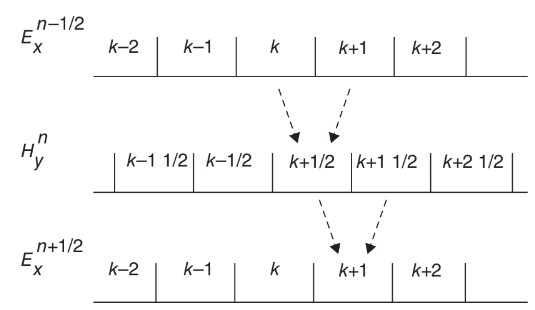
\includegraphics[scale=0.8]{Imagenes/Sullivan_interleaved.jpg}
    \caption{Interleaving of the electric and magnetic fields in the FDTD formulation. Image taken from \cite{Sullivan2020}.}
    \label{fig:sullivaninterleaved}
\end{figure}
\subsection{Boundary conditions}

We have seen that to evolve the field in a node we require the neighboring nodes of the other field, but then, what happens with the electric field in the nodes at the ends of the mesh? These nodes only have one neighbor magnetic field so it is not possible to apply the iterative formula of the FDTD algortihm. In order to compute the electric field at those positions, it is necessary to introduce boundary conditions, for example, the perfect electric conductor boundary condition states that the electric field on these nodes are equals to $0$ causing the electromagnetic wave to "bounce" when interacting with the ends of the mesh; another possible solution is the periodic boundary condition which are characterized as follows
\begin{equation}
    E_x^{n+1/2}(0) = E_x^{n-1/2}(0) - \dfrac{\Delta t}{\epsilon 0 \cdot \Delta x}\left[H_{y}^{n}\left(\frac{1}{2}\right)-H_{y}^{n}\left(N-\frac{1}{2}\right)\right],
\end{equation} 
where $N$ is the number of cells in the mesh and $E_x(N) = E_x(0)$ for all the time steps.

\section{Two dimensional discrete Maxwell equations}

In two dimensional problems, the third dimension is invariant \cite{peterson1992electromagnetic}, for this reason, it's convenient to separate the fields in two groups and only work with one of those; the first one is the transversal magnetic mode (TM), which is composed of $H_x$, $H_y$ and $E_z$, and the other group is the transversal electric mode (TE), composed of $E_x$, $E_y$ and $H_z$. In this work we only consider the TE mode.

\indent Considering again the time-dependent Maxwell's curl equations for the free space and by introducing the TE mode, we can obtain
\begin{align}
    \dfrac{\partial H_z}{\partial t} &= -\dfrac{1}{\mu_0} \left( \dfrac{\partial E_y}{\partial x} - \dfrac{\partial E_x}{\partial y} \right), \\
    \dfrac{\partial E_x}{\partial t} &= \dfrac{1}{\epsilon_0} \dfrac{\partial H_z}{\partial y}, \\
    \dfrac{\partial E_y}{\partial t} &= -\dfrac{1}{\epsilon_0} \dfrac{\partial H_z}{\partial x}. 
\end{align}
We can again use the central difference approximation but now with two spatial steps $\Delta x$ and $\Delta y$ to obtain the next iterive equation for the magnetic field
\begin{equation}
\begin{aligned}
    H_z^{n + 1}\left( i + \dfrac{1}{2},j + \dfrac{1}{2} \right) = H_z^{n}\left( i + \dfrac{1}{2},j + \dfrac{1}{2} \right) &- \dfrac{\Delta t}{\mu_0 \Delta x}\left( E_y^{n + 1/2}(i+1,j) - E_y^{n + 1/2}(i,j) \right) \\
                                                                                                                          &+ \dfrac{\Delta t}{\mu_0 \Delta y}\left( E_x^{n + 1/2}(i,j+1) - E_x^{n + 1/2}(i,j) \right),
\end{aligned}
\label{eq:FDTDMagneticField2D}
\end{equation}
and the next ones for the electric fields
\begin{align}
    E_x^{n+1}(i, j) &= E_x^{n}(i, j) + \dfrac{\Delta t}{\epsilon_0 \Delta y}\left[ H_z^{n+1/2}\left( i,j + \dfrac{1}{2} \right) - H_z^{n+1/2}\left( i,j - \dfrac{1}{2} \right) \right], \\
    E_y^{n+1}(i, j) &= E_x^{n}(i, j) + \dfrac{\Delta t}{\epsilon_0 \Delta x}\left[ H_z^{n+1/2}\left( i + \dfrac{1}{2},j \right) - H_z^{n+1/2}\left( i - \dfrac{1}{2},j \right) \right].
\end{align}

\section{Stability in the FDTD method}

We have seen that the central difference approximation used converges to the analytic solution with cuadratic order, in this case, we have errors similar to $\mathcal{O}(\Delta t(\Delta t^2 + \Delta x^2))$ in one dimension and $\mathcal{O}(\Delta t(\Delta t^2 + \Delta x^2 + \Delta y^2))$ in the two dimension case, however, there are some restrictions in order to guarantee the convergence.

\indent First let's start with the restriction of the time step $\Delta t$. The maximum value this parameter can have is determined by the \textit{CFL} condition, the physical meaning of this condition states that the electromagnetic wave must not pass through more than one cell in just one time step \cite{kunz1993finite}, and this have mathematical sense since the central difference approximation only consideres the nearest neighbors to estimate the evolution of the cell. In general, for a 3D rectangular grid, we have
\begin{equation}
    c \Delta t \leq \left( \dfrac{1}{(\Delta x)^2} + \dfrac{1}{(\Delta y)^2} + \dfrac{1}{(\Delta z)^2} \right)^{-1/2} \equiv d,
\end{equation}
where $c$ represents the speed of the electromagnetic wave (speed of light in the free space case). We can convert the inequality into an equality by multiplying by a constant $k$ less than 1 on the right side, so we finally have
\begin{equation}
    \Delta t = \dfrac{kd}{c}.
    \label{eq:CFL}
\end{equation}

Finally, the spatial step can not be selected at random either. The foundamental restriction is that the cell size must be smaller than the smallest wavelenght of the electromagnetic wave \cite{kunz1993finite}. A frequently used rule states that we need to have at least 10 cells per wavelenght.

\chapter{Conformal extension of the FDTD method}

Using the FDTD method with rectangular grid to analyze objects with curved metallic surfaces not only introduces errors due to inaccurate approximation of the geometry \cite{97384}. If we want to extend the FDTD method to solve curved surfaces or irregularities composed of perfect electric conductor, it's necessary to introduce the Conformal Finite Differece in Time Domain method (CFDTD). In this chapter we introduce the CFDTD basics.

\section{Introduction to CFDTD}

The CFDTD algorithm was first introduced to made a FDTD analysis of a curved two dimensional PEC using a locally conformal grid \cite{DeyMittra1997}. For two dimensional problems we can consider for example a quadrant of the cross section of a circular resonator shown in Figure \ref{fig:DeyMittraMesh}; we can see that the magnetic fields over the cells that don't intersects with the curve can be solved with the regular FDTD method, however, we can't use the same algorithm for the others cells; this is because some neighbour nodes of the electric field discretization are no longer able to interact due to the presence of the PEC surface between them. For this reason, we need to introduce another formulation for the FDTD that can be generalized and used for the CFDTD case.

\begin{figure}[h]
    \centering
    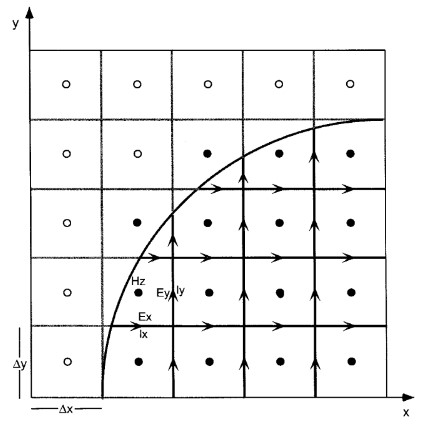
\includegraphics[scale=1.0]{Imagenes/DeyMittra_2DMeshExample.jpg}
    \caption{Example of a rectangular mesh on a curved PEC surface. Image taken from \cite{Dey1997ALC}.}
    \label{fig:DeyMittraMesh}
\end{figure}

\section{The Dey-Mittra algorithm}

Let's consider a two dimensional rectangular grid discretization same as the FDTD case. Now, let's consider the Faraday equation in the integral form for the free space given by
\begin{equation}
    \oint_{\partial S} \boldsymbol{E} \cdot d \boldsymbol{l} = -\dfrac{d}{dt} \int_{S} \mu_0 \boldsymbol{H} \cdot d\boldsymbol{s}.
    \label{eq:FaradayIntegralEquation}
\end{equation}
If we assume that the electric fields are constant along the edges between the nodes, that the magnetics fields are also constant in the worked cell and if we are working on the TE mode, we can obtain from the equation \ref{eq:FaradayIntegralEquation} the following relation
\begin{equation}
\begin{aligned}
    -\mu_0 \cdot A(i,j)\dfrac{\partial}{\partial t} H_z\left( i + \dfrac{1}{2}, j + \dfrac{1}{2} \right) &= E_x(i,j)\cdot l_x(i,j) - E_x(i,j+1) \cdot l_x(i,j+1) \\
                                                                                                   &+ E_y(i+1,j)\cdot l_y(i+1,j) - E_y(i,j)\cdot l_y(i,j),  
\end{aligned}
\label{eq:FaradayIntegralEquationRectangularGrid}
\end{equation}
where $l_x(i,j)$ and $l_y(i,j)$ represents the length of the edge where is assumed the electric node $E_x(i,j)$ and $E_y(i,j)$ respectively, and $A(i,j)$ the area where the magnetic field $H_z (i + 1/2, j + 1/2)$ is placed. We also assumed that the area is constant in the time so it can separated from the time derivative. Finally we take the central difference aproximation for the time derivative and rearranging we obtain
\begin{equation}
    \begin{aligned}
        H_z^{n + 1}\left( i + \dfrac{1}{2}, j + \dfrac{1}{2} \right) &= H_z^{n}\left( i + \dfrac{1}{2}, j + \dfrac{1}{2} \right)  \\
        - \dfrac{\Delta t}{\mu_0 \cdot A(i,j)} & \big[ E^{n + 1/2}_x(i,j)\cdot l_x(i,j)- E^{n + 1/2}_x(i,j+1)\cdot l_x(i,j+1)  \\
                                                                       &+  E^{n + 1/2}_y(i+1,j)\cdot l_y(i+1,j) - E^{n + 1/2}_y(i,j)\cdot l_y(i,j)\big].  
    \end{aligned}
\label{eq:FaradayIntegralEquationRectangularGrid}
\end{equation}

In the uniform rectangular grid case, if there is no curved surface in the mesh, we have $l_x = \Delta x$, $l_y = \Delta y$ and $A = \Delta x \Delta y$ for any pair $i,j$, then, by replacing these values into the equation \ref{eq:FaradayIntegralEquationRectangularGrid}, we can obtain again the magnetic field iterative formula presented in the equation \ref{eq:FDTDMagneticField2D}.

The great advantage of this formulation is the fact that we can use it to solve curved PEC surfaces with rectangular grids like the one shown in the Figure \ref{fig:DeyMittraMesh}. Indeed, as said before, the cells thats don't intersect with the curved surface can be solved as stated, on the other hand, in cells with non-empty intersections, we need to consider in the path integral of the electric field another component corresponding to the value of this field over the part of the curved surface inside the cell, however, the field over this path is always zero, for this reason, the construction of the iterative formula of the magnetic field remains valid, but it must be taken into account that the lengths and areas in these cells doesn't have the usual values now. This formulation is knowed as the Dey-Mittra algorithm in two dimensions \cite{DeyMittra1997}.

\section{Stability in the CFDTD method}

As we have seen, the CFDTD method follows a different scheme that the FDTD method in the cells where the curved PEC surface intersects the mesh, since the area and the lengths of some cells changes, we need to find a stability that depends on these variables, then, we need a more restrictive time step stability condition. For example, the condition reported in \cite{7518629} establish that
\begin{equation}
    \Delta t_k = \sqrt{3} \sqrt{\dfrac{A_k^{ratio}}{\max \left( l_k^{ratio} \right)}}\Delta t_{CFL} = h_{0, k} \Delta t_{CFL},
\label{eq:StabilityAngulo}
\end{equation}
with $h_{0, k} = \sqrt{3} \sqrt{A_k^{ratio}/\max \left( l_k^{ratio} \right)} \leq 1$. In this equation $k$ represents one of the posibles remaining areas when we consider the cell cut by the curve, $A^{ratio}$ represent the quotient between the remaining area from the usual area of the cell and $l^{ratio}$ the quotient between the cut length of the edge from the usual length (considering al the four posible lengths per cell). This time step is similar to the time step reported in \cite{1638381}, the only difference is the factor $\sqrt{3}$, however, both of these criterias are made for 3D problems, in case we want to work with 1D or 2D problems, we can change the previously factor to $1$ or $\sqrt{2}$ respectively.

Returning to the equation \ref{eq:StabilityAngulo}, there is a problem with this formulation, to guarantee the stability of the scheme, we need to look over all the cells of the discretization, making the algorithm inefficient or slow for large problems with short spatial step or problems with complex geometries that require very detailed refinement of the mesh. For this reason, the study of local stability conditions that require only specific information about the problem has been a research objective for both CFDTD and FDTD \cite{7779120}.

\chapter{CFDTD implementation and results}

In this section, we discuss the CFDTD method implementation along some results that we compare with the literature.
\section{One dimensional CFDTD}
Let's start with the formalism in one dimension. In this case, it is impossible to consider a curved PEC surface because of the dimensions of the mesh, so how can we formulate a 1D CFDTD algorithm? Before thinking about the iterative formula, it is necessary to see that the equivalent of the curved surface in this case is equal to a PEC sheet between two nodes of the mesh as we can see in the Figure \ref{fig:Mesh1D_CFDTD}, following this, we can separate the nodes of the mesh in two groups, the first one being those nodes $n_i$ in such a way that the PEC sheet it's not contained in the intervals $(n_{i-1}, n_i)$ or $(n_i, n_{i+1})$; the second group being those nodes that are "neighbors" of the PEC sheet. 
\begin{figure}[h]
    \centering
    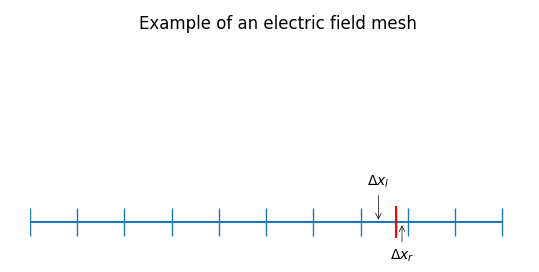
\includegraphics[scale=0.8]{Imagenes/Mesh1D_CFDTD.png}
    \caption{Example of an uniform mesh for the electric field in one dimension (blue dots) with a PEC sheet between two nodes (red dot).}
    \label{fig:Mesh1D_CFDTD}
\end{figure}

In the first group of nodes (the non frontier nodes), for both the electric and magnetic field, we can again use the usual FDTD iterative formula because the distance between neighboring nodes remains equal to $\Delta x$. However, for the neighbor nodes of the PEC sheet, we need to change the iterative equations because the existence of the irregularity, in order to formulate a possible solution, we can consider the PEC sheet position like another node of the electric field mesh adding one degree of freedom to the magnetic and electric field solution (remembering that the solution of the electric field must be equal to zero at all times in this extra node); with this in mind, we can use a linear interpolation in order to formulate a valid iterative formula, then, if $k_p$ represents the PEC sheet node in the electric field mesh, we have the following equations
\begin{align}
    H_y^{n+1} \left( k_p - \dfrac{1}{2} \right) &= H_y^{n} \left( k_p - \dfrac{1}{2} \right) + \dfrac{\Delta t}{\mu_0 \Delta x_l}E_x^{n+1/2}(k_p - 1), \\
    H_y^{n+1} \left( k_p + \dfrac{1}{2} \right) &= H_y^{n} \left( k_p + \dfrac{1}{2} \right) - \dfrac{\Delta t}{\mu_0 \Delta x_r}E_x^{n+1/2}(k_p + 1), \\
    E_x^{n+1/2}(k_p - 1) &= E_x^{n-1/2}(k_p - 1) - \dfrac{\Delta t}{\epsilon_0 \Delta x_l} \left[  H_y^{n} \left( k_p + \dfrac{1}{2} \right) -  H_y^{n} \left( k_p - \dfrac{1}{2} \right) \right], \\
    E_x^{n+1/2}(k_p + 1) &= E_x^{n-1/2}(k_p + 1) - \dfrac{\Delta t}{\epsilon_0 \Delta x_r} \left[  H_y^{n} \left( k_p + \dfrac{3}{2} \right) -  H_y^{n} \left( k_p + \dfrac{1}{2} \right) \right].
\end{align}
Where $\Delta x_l + \Delta x_r = \Delta x$ represents the existing distance between the PEC sheet node to the left and right node respectively. With these equations already formulated, we can start with the study and validation of our implementation; the electromagnetic wave to study is a Gaussian pulse defined by the initial pulse
\begin{align}
    E_0 (k_0) &= \Delta t * exp \left[-0.5 \left( \dfrac{t_0 - n \Delta t}{s} \right)^2 \right], \\
    H_0 (k_0) &= \Delta t * exp \left[-0.5 \left( \dfrac{t_0 - n \Delta t - \dfrac{\Delta t}{2} - \dfrac{\Delta x}{2c}}{s} \right)^2 \right],
\end{align}
where $s$ is the spread of the wave, $t_0$ the initial time and $n$ the current step of the simulation; in order to simplify the algorithm, we also work with natural units ($c=1$). The python script used to recreate the CFDTD algorithm in one dimension and the tests associated can be found in the attached GitHub repository in the files \textit{cfdtd/CFDTD1D.py} and \textit{test/test\_1D.py} respectively. The first result that is expected to be observed is the instability of the solution with some Courant numbers (the constant $k$ in the equation \ref{eq:CFL}) when the PEC sheet node doesn't match with any other node of the mesh, indeed, we can consider a mesh of length equals to $200$ and spatial step $\Delta x = 1.0$ and a PEC sheet positioned at $150.5$; if the behavior of the CFDTD algorithm were the same as that of the FDTD, we expect the solution of the fields to be stable at all time steps, however, this doesn't happen as we can see in the Figure \ref{fig:CFDTD1D_Inestability}.
\begin{figure}[h!]
    \centering
    \begin{subfigure}[b]{0.49\textwidth}
        \centering
        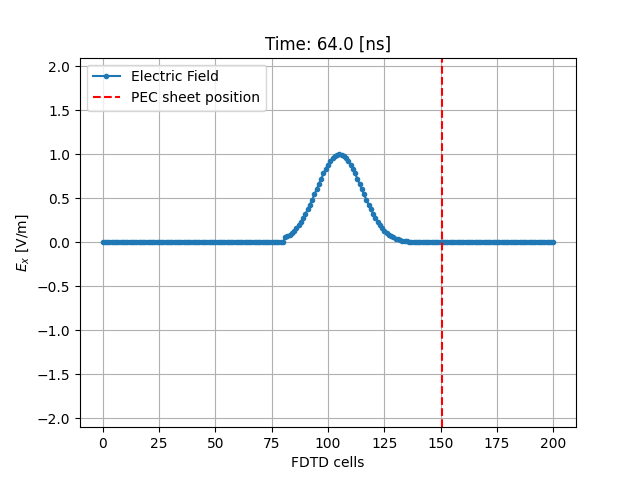
\includegraphics[width=\textwidth]{Imagenes/CFDTD1D_Inestibility1.png}
    \end{subfigure}
    \begin{subfigure}[b]{0.49\textwidth}
        \centering
        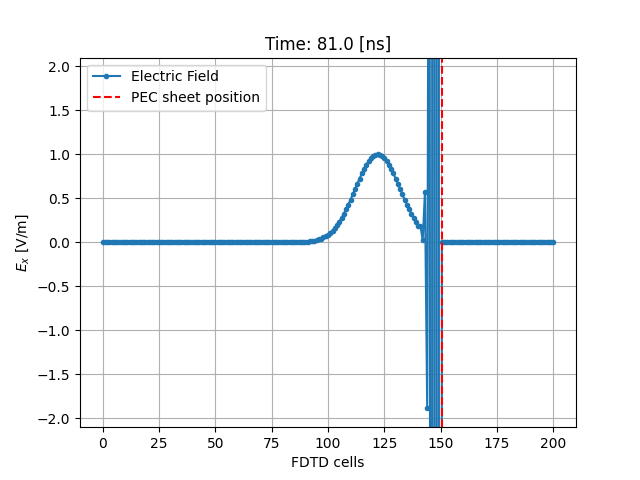
\includegraphics[width=\textwidth]{Imagenes/CFDTD1D_Inestibility2.png}
    \end{subfigure}
    \caption{Propagation of the Gaussian electromagnetic wave with PEC boundary conditions and Courant number equals to $1.0$ in different time steps, on the left in step 65 and on the right in step 80.}
    \label{fig:CFDTD1D_Inestability}
\end{figure}

We can also make a comparison between a FDTD solution with PEC boundary conditions and a CFDTD solution with also PEC boundary conditions but with the PEC sheet position located $0.5$ before the right end of the mesh, we expect to see a delay of the non conformal solution with respect to the conformal solution just after bouncing the PEC sheet, this delay should increase depending on the number of times the wave has interacted with the PEC surface, as seen in the Figure \ref{fig:CFDTD1D_Delay}. In particular, we can corroborate that the conformal solution after two bounces is the same as the non conformal one but moved two nodes as can be found in the respective test and in the figure \ref{fig:CFDTD1D_DelayNorm}. 

\begin{figure}[h!]
    \centering
    \begin{subfigure}[b]{0.49\textwidth}
        \centering
        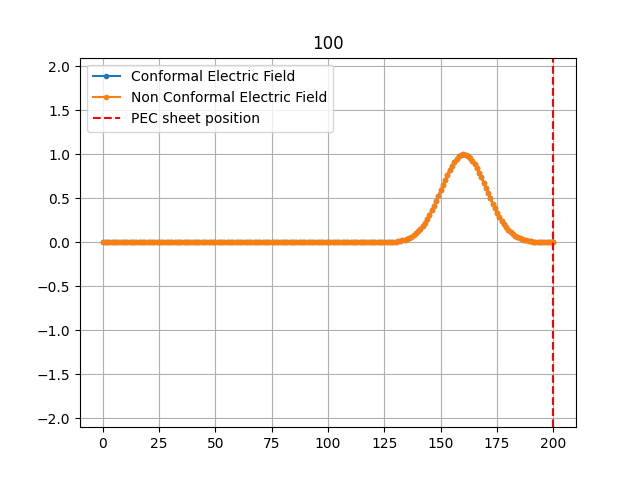
\includegraphics[width=\textwidth]{Imagenes/CFDTD1D_Comparison1.png}
    \end{subfigure}
    \begin{subfigure}[b]{0.49\textwidth}
        \centering
        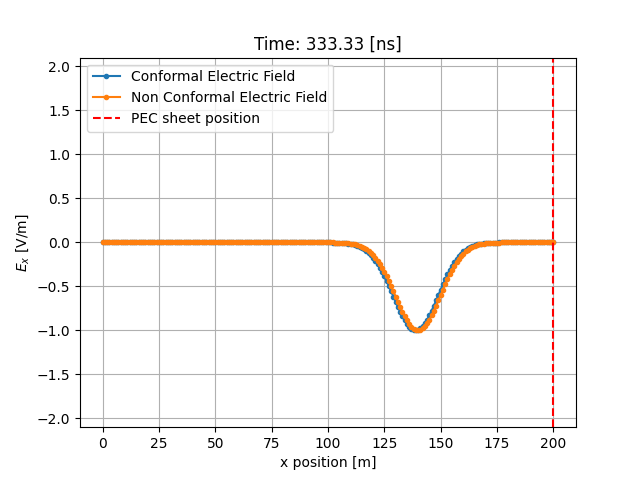
\includegraphics[width=\textwidth]{Imagenes/CFDTD1D_Comparison2.png}
    \end{subfigure}

    \vskip\baselineskip
    
    \begin{subfigure}[b]{0.49\textwidth}
        \centering
        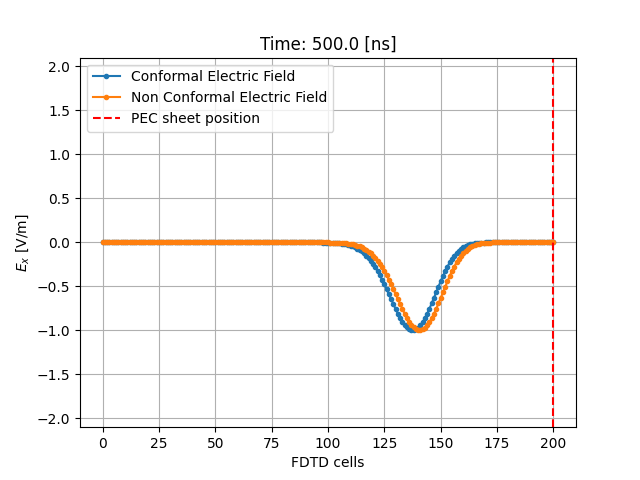
\includegraphics[width=\textwidth]{Imagenes/CFDTD1D_Comparison3.png}
    \end{subfigure}
    \begin{subfigure}[b]{0.49\textwidth}
        \centering
        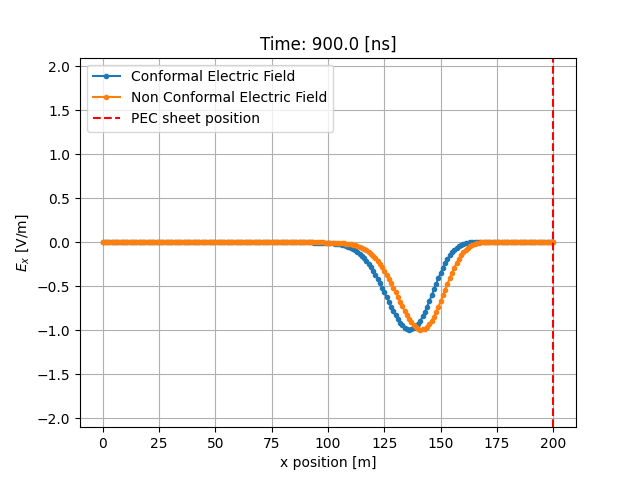
\includegraphics[width=\textwidth]{Imagenes/CFDTD1D_Comparison4.png}
    \end{subfigure}
    \caption{Comparison between conformal and non conformal solutions of the Gaussian electromagnetic wave in different time steps.}
    \label{fig:CFDTD1D_Delay}
\end{figure}

\begin{figure}[h!]
    \centering
    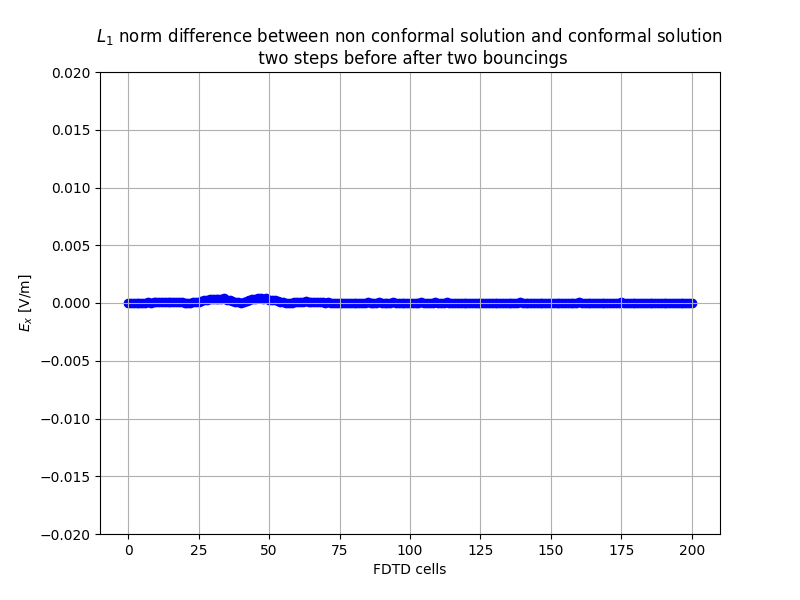
\includegraphics[scale=0.6]{Imagenes/CFDTD1D_DelayNorm.png}
    \caption{$L_1$ norm difference between non conformal solution and conformal solution two steps before after two bouncings with the PEC sheet.}
    \label{fig:CFDTD1D_DelayNorm}
\end{figure}
\newpage
\section{Two dimensional CFDTD}

Now, unlike the previous case, the CFDTD algorithm in more than one dimension becomes more complicated because there is more freedom in the election of the PEC surface inside the mesh. For this and other reasons, it is necessary to carry out a study on the geometry of the problem before entering the CFDTD-2D algorithm.

\subsection{Mesh geometry}

Returning to the formulation of the Dey-Mittra algorithm, the difference between the CFDTD and FDTD method lies in the areas and lengths of the cells, so for example, if the curved surface intersects one cell, we need the coordinates of the intersection points to estimate the value of the respective length, for this reason, the coordinates of all existing intersenctions play an important role in the development of the algorithm.

In some of the codes that have been worked around the FDTD method in two dimensions (such as \cite{Angulo_PyDG1D_2024}), the mesh is obtained through a "\textit{meshgrid}" function \cite{harris2020array} which takes as argument the two 1D spatial meshes with spatial steps $\Delta x$ and $\Delta y$. If we want to work similar to the one dimension algortihm, it is necessary to add a number of extra nodes corresponding to the intersection points to the mesh, but what happens if we want to add an extra node to the meshgrid? The answer to this can be seen in the Figure \ref{fig:CFDTD2D_Meshgrid} where we can see that adding just one extra node introduces a number of unused nodes equal to the number of points contemplated by the 1D mesh where said node is not located; this causes us to go from $N_x \times N_y$ points to a total of $(N_x + M_x) \times (N_y + M_y)$ increasing the complexity of the system, where $N_x$ and $N_y$ are the number of nodes of the 1D meshes and $M_x + M_y = M$ is the number of intersection points that can belong to one of the two meshes. 

\begin{figure}[h!]
    \centering
    \begin{subfigure}[b]{0.49\textwidth}
        \centering
        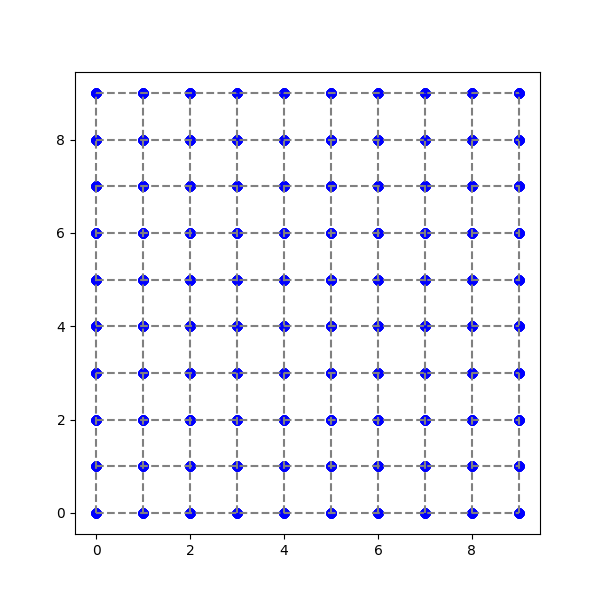
\includegraphics[width=\textwidth]{Imagenes/CFDTD2D_Meshgrid1.png}
    \end{subfigure}
    \begin{subfigure}[b]{0.49\textwidth}
        \centering
        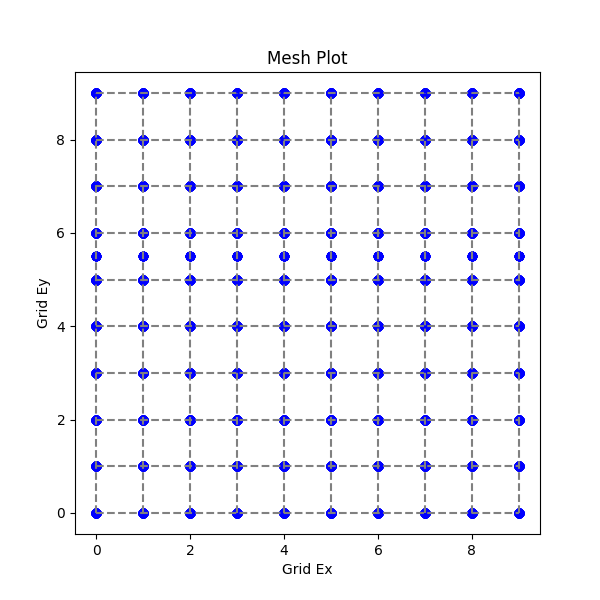
\includegraphics[width=\textwidth]{Imagenes/CFDTD2D_Meshgrid2.png}
    \end{subfigure}
    \caption{Meshgrid function in python before (left) and after (right) adding as an extra node the point $(5, 5.5)$.}
    \label{fig:CFDTD2D_Meshgrid}
\end{figure}

In order to avoid this problem, we propose another way of working with the mesh using polygons and the python library "\textit{shapely}" \cite{Gillies_Shapely_2024}, instead of working with all the nodes of the 2D meshgrid with all the intersection points, we characterize the mesh with a total of $(N_x - 1) \times (N_y - 1)$ polygons that represent all the cells contained in the mesh and another polygon used to represent the PEC surface, in this way, it is possible to calculate the lengths and areas of each cell using Boolean operations. 

To simplify the problem worked on, we restrict the PEC surface to be a line or a polygon that separates a maximum of one cell into two cells, the intersection points of a cell must be zero or two depending on wether the intersection between the cell and the PEC polygon is empty or not, an example of the 2D mesh with a PEC polygon or PEC line is presented in the Figure \ref{fig:CFDTD2D_MeshPEC}. With this in mind, if we work with a PEC line we can separate the cells in two groups depending on the number of intersection points: the conformal cells with a number of intersections equal to $2$ and the non conformal cells with empty intersection; in a similar way, for the PEC polygon we can separate the cells in three groups: the conformal cells and the outside or inside non conformal cells, the latter depending on whether they are inside or outside the PEC polygon.

\begin{figure}[h!]
    \centering
    \begin{subfigure}[b]{0.49\textwidth}
        \centering
        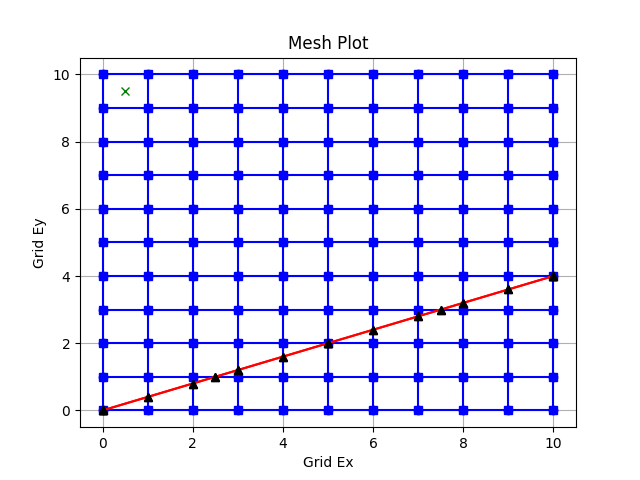
\includegraphics[width=\textwidth]{Imagenes/CFDTD2D_MeshPECLine.png}
    \end{subfigure}
    \begin{subfigure}[b]{0.49\textwidth}
        \centering
        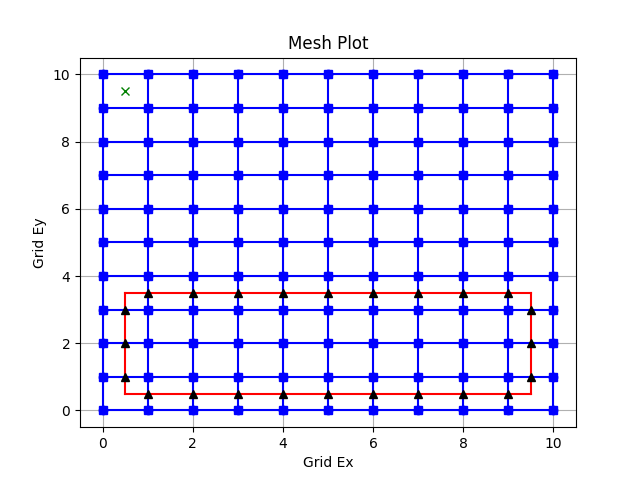
\includegraphics[width=\textwidth]{Imagenes/CFDTD2D_MeshPECPolygon.png}
    \end{subfigure}
    \caption{Two dimensional mesh (blue dots) considering a PEC line (left) or a PEC polygon (right) represented by the red line, the intersection points are identified as the black triangular marker, the green cross marker represents a reference cell for the initial wave.}
    \label{fig:CFDTD2D_MeshPEC}
\end{figure}

Finally, a separation is made so that the mesh knows whether to interpret the lengths or areas depending on whether the wave to be solved is inside or outside the PEC polygon (the option of solving both regions at the same time is excluded). The mesh creation algorithm can be found in the file \textit{mesh/MESH2D.py} and to guarantee its correct functioning, various tests are carried out such as: that the groups in which the cells are separated are mutually exclusive and the sum of its elements is equal to the total number of cells, that the area of non conformal cells are equal to $\Delta x \Delta y$, that the lengths of non conformal cells are equal to $\Delta x$ or $\Delta y$ and that the sum of lengths of the two cells into which a conformal cell is divided also meets the same previous equality, etc; all of these tests can be found in the file \textit{test/test\_Mesh\_2D.py}. 

The great advantage of the constructed algorithm is its ease of being adapted to any curved PEC surface; it is only necessary to introduce as an argument a list of points corresponding to the intersection points of the curve with the mesh for the construction of the PEC polygon. The difference between working with the curved surface and the polygon is that the areas of the cell can be different, however, for a sufficiently dense mesh, this difference is minimal.

\subsection{Two dimensional algorithm}

Once the mesh is built, adapting it to the Dey-Mittra algorithm is relatively easy, it is only necessary to pass the mesh as an argument and when performing the time steps of the electromagnetic fields, call the area and length calculation routine defined in the mesh script for the worked cell. 

For the validation of the method, we consider three different possible initial pulses for the electromagnetic wave, these being the two dimensional Gaussian, the Gaussian restricted to one dimension and the resonant rectangular cavity in the mode $44$; all of these can be found in the python script "\textit{initial\_pulse/INITIAL\_PULSE2D.py}", this class needs as arguments the spread of the wave, the mesh worked, the same reference cell mentioned in the previous subsection and the type of the pulse to work. Once we have defined our mesh and initial pulse, we can start our solver which needs as arguments the two previously mentioned classes and the Courant number. The solver class can be found in the file "\textit{cfdtd/CFDTD2D.py}".

We begin our validation, seeing at the solution obtained from a Gaussian magnetic wave that depends only on the $x$ coordinate as follows
\begin{equation}
    H_{0z}(x,y) = \exp \left[ - \dfrac{(x - x_0)^2}{\sqrt{2} s} \right],
\label{eq:EyInitialCondition}
\end{equation}
where $x_0$ is the first coordinate of the reference cell and $s$ is the spread of the wave. We work with a square mesh of dimensions $100 \times 100$ and spatial steps $\Delta x = \Delta y = 2.0$, inside this mesh we put a rectangular PEC polygon defined by the nodes $(5.5,40.5)$, $(94.5,40.5)$, $(94.5, 60.5)$ and $(5.5, 60.5)$ and we take $(50, 50)$ as the reference cell; then, we put the initial condition defined in equation \ref{eq:EyInitialCondition} inside the PEC polygon and start the solver with a Courant number equals to $0.4$. With these parameters, we expect the evolution of the wave to have a similar behavior as if it were in one dimension, i.e., it only propagates in one direction. The result of our simulation is represented in figure \ref{fig:CFDTD2D_GaussianEy} where the expected behavior is confirmed.

\begin{figure}[h!]
    \centering
    \begin{subfigure}[b]{0.49\textwidth}
        \centering
        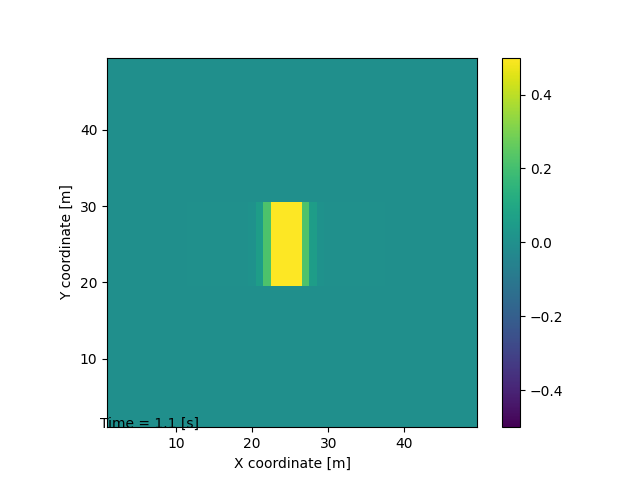
\includegraphics[width=\textwidth]{Imagenes/CFDTD2D_GaussianY1.png}
    \end{subfigure}
    \begin{subfigure}[b]{0.49\textwidth}
        \centering
        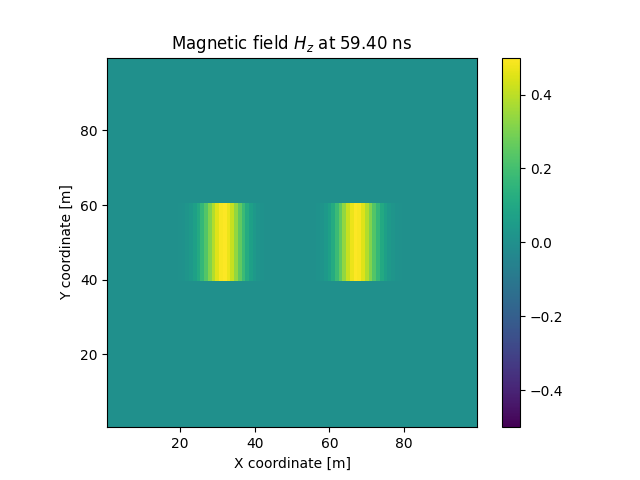
\includegraphics[width=\textwidth]{Imagenes/CFDTD2D_GaussianY2.png}
    \end{subfigure}

    \vskip\baselineskip
    
    \begin{subfigure}[b]{0.49\textwidth}
        \centering
        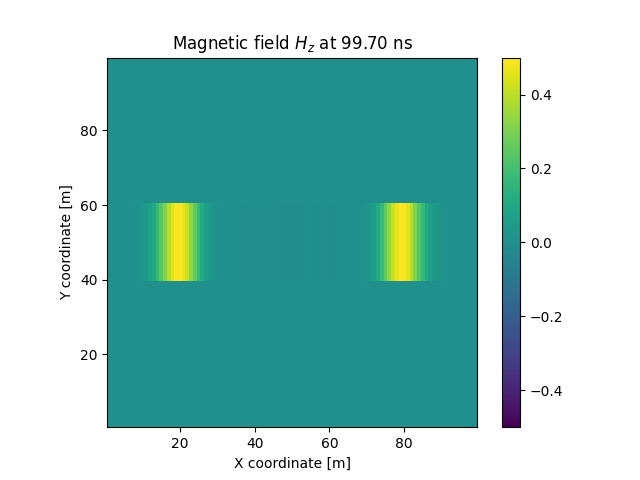
\includegraphics[width=\textwidth]{Imagenes/CFDTD2D_GaussianY3.png}
    \end{subfigure}
    \begin{subfigure}[b]{0.49\textwidth}
        \centering
        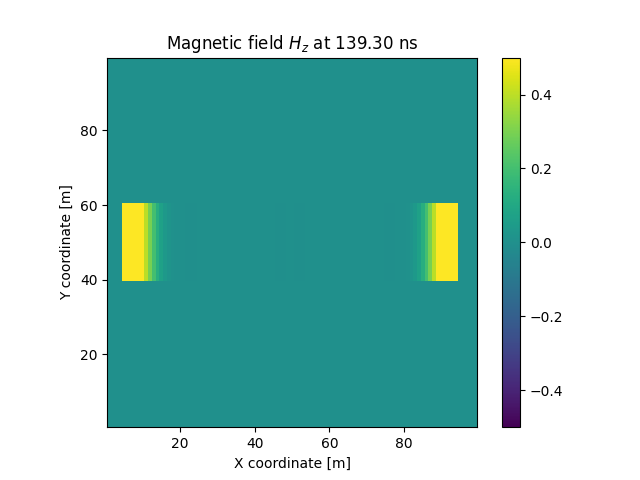
\includegraphics[width=\textwidth]{Imagenes/CFDTD2D_GaussianY4.png}
    \end{subfigure}
    \caption{Evolution of a Gaussian pulse defined by equation \ref{eq:EyInitialCondition} inside a rectangular PEC polygon with CFDTD.}
    \label{fig:CFDTD2D_GaussianEy}
\end{figure}
\newpage
Next we want to study the stability of a initial Gaussian magnetic wave defined by 
\begin{equation}
    H_{0z}(x,y) = \exp \left[ - \dfrac{(x - x_0)^2 + (y - y_0)^2}{\sqrt{2} s} \right],
\label{eq:Gaussian2DInitialCondition}
\end{equation}
if we work with a mesh similar to the previous one used but now with $\Delta x = \Delta y = 1.0$, and a rectangular PEC polygon defined by the nodes $(25.5,10.5)$, $(75.5,10.5)$, $(75.5, 95.5)$ and $(25.5, 95.5)$. In this case, we have two tipes of conformal cells, the cells that have $A^{ratio} = 1/4$ and $\max({l^{ratio}}) = 1/2$ (the corner conformal cells); and the cells that have $A^{ratio} = 1/2$ and $\max({l^{ratio}}) = 1$, following the equation \ref{eq:StabilityAngulo}, we observe in both cases that $\Delta t = \Delta t_{CFL}$, so we expect not to observe any instability for any Courant number less or equal to $1$ as seen in the Figure \ref{fig:CFDTD2D_GaussianStability}. On the other hand, if we replace $10.5$ with $10.6$ and $95.5$ with $95.4$ in the nodes of the PEC polygon, we obtain $A^{ratio} = 1/5$ and $\max({l^{ratio}}) = 1/2$ for the corner conformal cells, then, for this cells we have $\Delta t \neq \Delta t_{CFL}$ and we expect to have numerical instability for Courant Number Equal to 1 as shown in Figure \ref{fig:CFDTD2D_GaussianInstability}.

\begin{figure}[h!]
    \centering
    \begin{subfigure}[b]{0.49\textwidth}
        \centering
        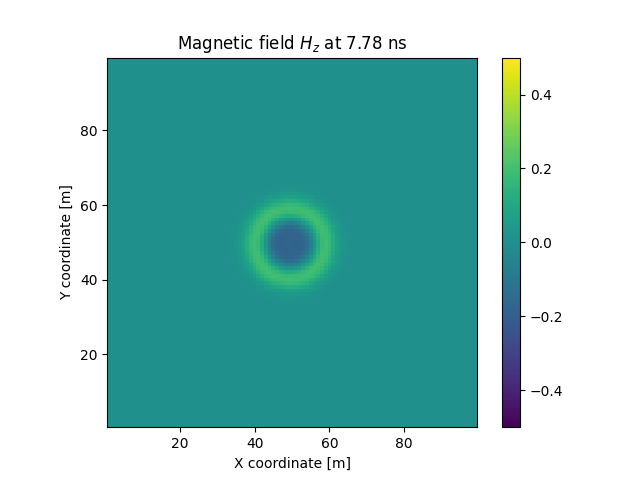
\includegraphics[width=\textwidth]{Imagenes/CFDTD2D_GaussianStability1.png}
    \end{subfigure}
    \begin{subfigure}[b]{0.49\textwidth}
        \centering
        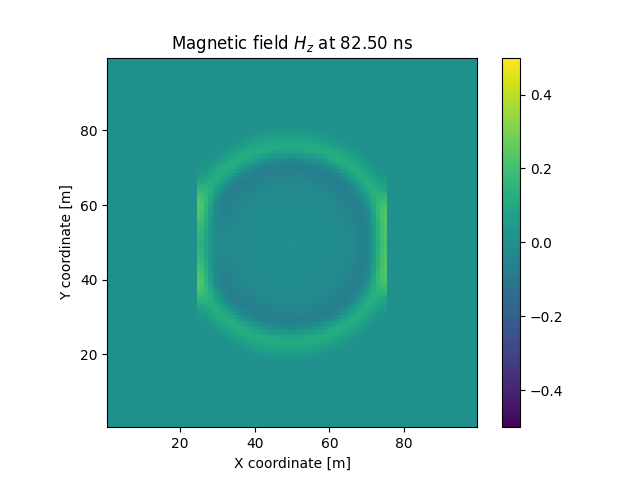
\includegraphics[width=\textwidth]{Imagenes/CFDTD2D_GaussianStability2.png}
    \end{subfigure}

    \vskip\baselineskip
    
    \begin{subfigure}[b]{0.49\textwidth}
        \centering
        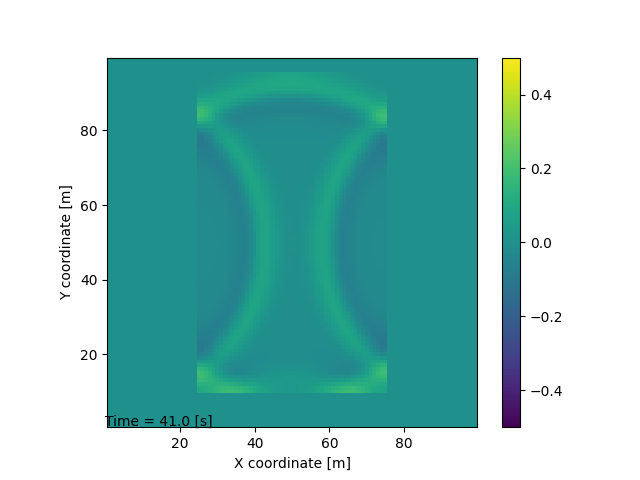
\includegraphics[width=\textwidth]{Imagenes/CFDTD2D_GaussianStability3.png}
    \end{subfigure}
    \begin{subfigure}[b]{0.49\textwidth}
        \centering
        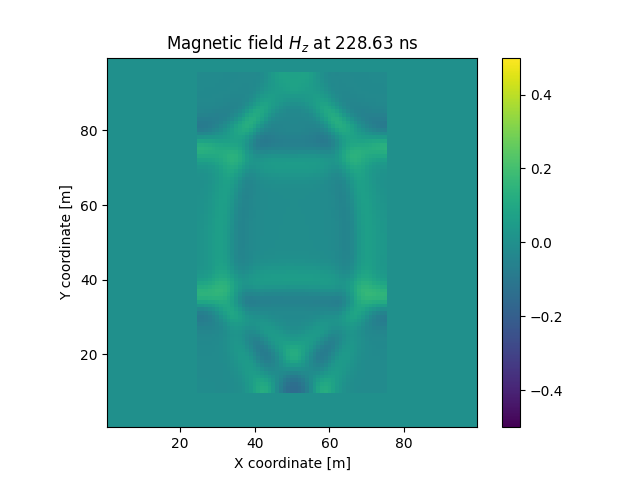
\includegraphics[width=\textwidth]{Imagenes/CFDTD2D_GaussianStability4.png}
    \end{subfigure}

    \vskip\baselineskip
    
    \begin{subfigure}[b]{0.49\textwidth}
        \centering
        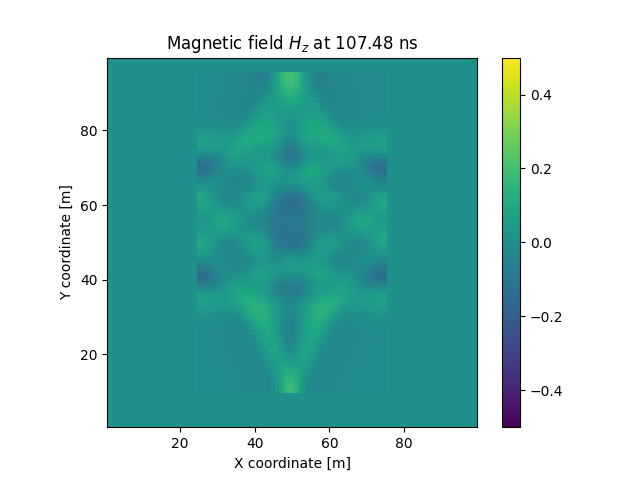
\includegraphics[width=\textwidth]{Imagenes/CFDTD2D_GaussianStability5.png}
    \end{subfigure}
    \begin{subfigure}[b]{0.49\textwidth}
        \centering
        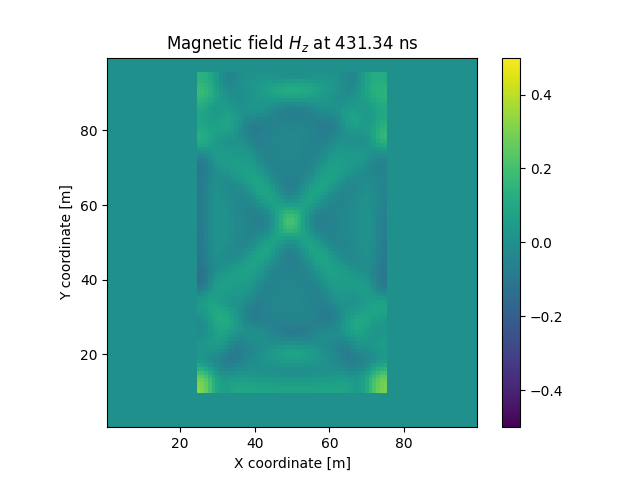
\includegraphics[width=\textwidth]{Imagenes/CFDTD2D_GaussianStability6.png}
    \end{subfigure}
    \caption{Evolution of a Gaussian 2D magnetic pulse defined by equation \ref{eq:Gaussian2DInitialCondition} inside a rectangular PEC polygon with $\Delta t = \Delta t_{CFL}$ and Courant number equal to $1.0$.}
    \label{fig:CFDTD2D_GaussianStability}
\end{figure}

\begin{figure}[h!]
    \centering
    \begin{subfigure}[b]{0.49\textwidth}
        \centering
        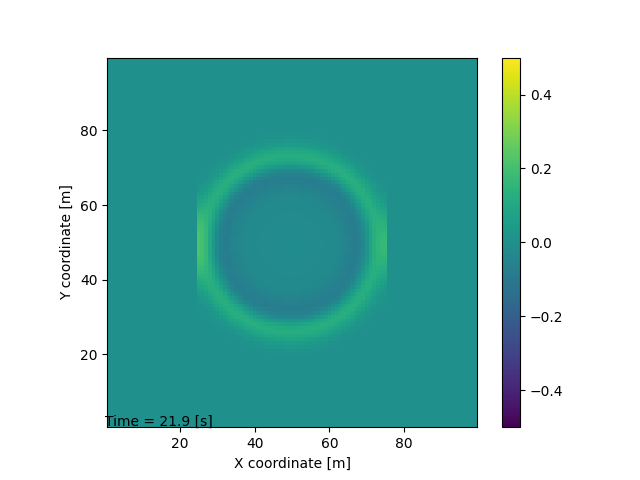
\includegraphics[width=\textwidth]{Imagenes/CFDTD2D_GaussianInstability1.png}
    \end{subfigure}
    \begin{subfigure}[b]{0.49\textwidth}
        \centering
        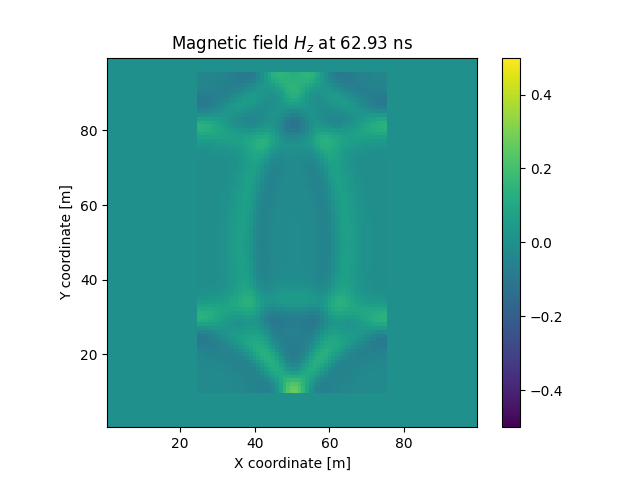
\includegraphics[width=\textwidth]{Imagenes/CFDTD2D_GaussianInstability2.png}
    \end{subfigure}

    \vskip\baselineskip
    
    \begin{subfigure}[b]{0.49\textwidth}
        \centering
        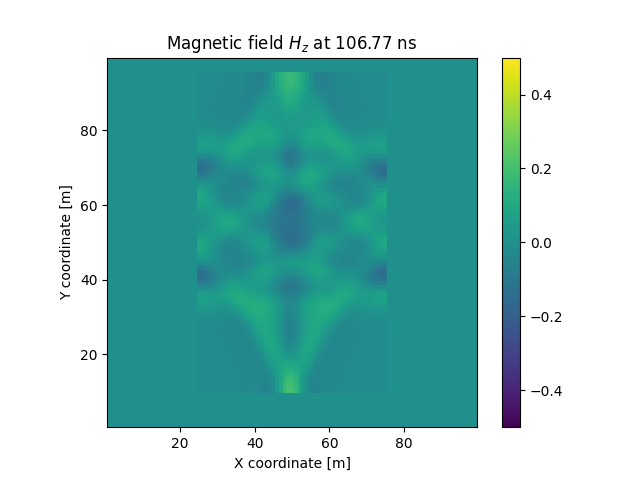
\includegraphics[width=\textwidth]{Imagenes/CFDTD2D_GaussianInstability3.png}
    \end{subfigure}
    \begin{subfigure}[b]{0.49\textwidth}
        \centering
        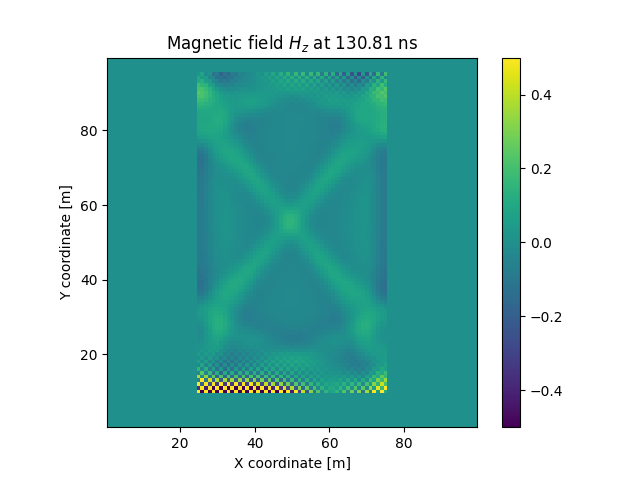
\includegraphics[width=\textwidth]{Imagenes/CFDTD2D_GaussianInstability4.png}
    \end{subfigure}
    \caption{Evolution of a Gaussian 2D magnetic pulse defined by equation \ref{eq:Gaussian2DInitialCondition} inside a rectangular PEC polygon with $\Delta t \neq \Delta t_{CFL}$ and Courant number equal to $1.0$. Instability starts to appear arround $130$ [s].}
    \label{fig:CFDTD2D_GaussianInstability}
\end{figure}
\newpage
Finally, we can also study the evolution of a electromagnetic wave inside a rectangular resonant cavity whose initial condition for the TE mode is given by \cite{pozar2012microwave}
\begin{equation}
    H_z(x, y) = A_{mn}\cos\dfrac{m \pi (x-x_0)}{a} \cos\dfrac{n \pi (y-y_0)}{b},
\label{eq:ResonantRectangularCavity}
\end{equation}
where $a$ and $b$ are the lengths of the rectangular box, $(x_0, y_0)$ is the lower left coordinate of the box, $m, n$ are positive integers and $A_{mn}$ is the amplitude of the wave. For the simulation, we again construct a mesh equal to the case of the 2D Gaussian, and a rectangular PEC polygon defined by the nodes $(10.5,10.5)$, $(95.5,10.5)$, $(95.5, 95.5)$ and $(10.5, 95.5)$, we again define the initial wave inside the PEC polygon. In particular, the wave we simulate is the mode $m = n = 4$, we expect to observe a resonance and periodic behavior in all the electromagnetic fields, and in fact, it is shown in the Figure \ref{fig:CFDTD2D_RectangularResonantCavity}.

\begin{figure}[h!]
    \centering
    \begin{subfigure}[b]{0.49\textwidth}
        \centering
        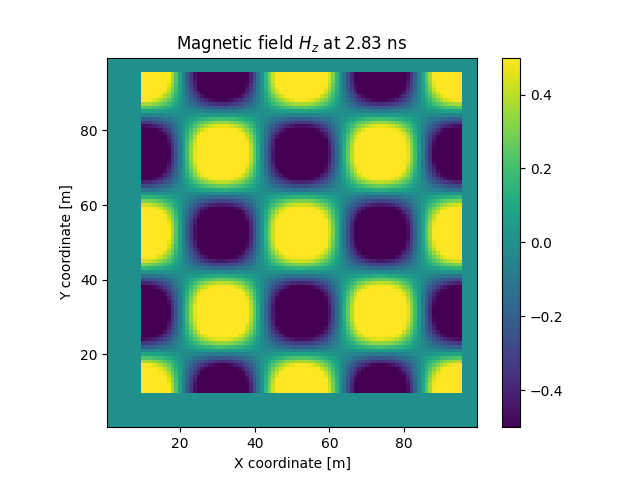
\includegraphics[width=\textwidth]{Imagenes/CFDTD2D_ResonantRectangularCavity1.png}
    \end{subfigure}
    \begin{subfigure}[b]{0.49\textwidth}
        \centering
        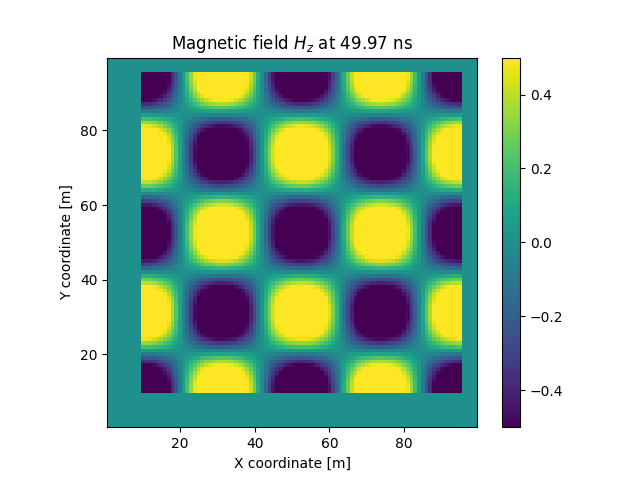
\includegraphics[width=\textwidth]{Imagenes/CFDTD2D_ResonantRectangularCavity2.png}
    \end{subfigure}
    \caption{Evolution of the magnetic wave defined by the equation \ref{eq:ResonantRectangularCavity} inside a square PEC using CFDTD. The evolution of the wave consists of transitions between the left state and the right state.}
    \label{fig:CFDTD2D_RectangularResonantCavity}
\end{figure}


\chapter{Conclusions}

In this work, a review and implementation of conformal finite differences in the time domain in both one and two dimensions was carried out, proposing for the first case an iterative formula based on an interpolation. It is verified that the conformal solution of a Gaussian presents a delay with respect to the non conformal solution when the PEC sheet is 0.5 units before the end of the mesh, finding in particular that after two bounces, the conformal wave is practically equal to the non conformal solution but with a two time steps difference.

For the two-dimensional case, a Python class was built for meshing where instead of interpreting the grid by nodes, it is interpreted through polygons in order to reduce the complexity of the problem for problems with large geometries. In order to guarantee the correct operation of the routines of this class, several tests were developed to check and verify the proper behavior in particular cases.

The Dey-Mittra algorithm was implemented in order to adapt the two dimensional solver to solve problems requiring CFDTD, the evolution of a "1.5 "D Gaussian pulse was studied to observe behaviors similar to the evolution of a 1D Gaussian wave. The stability behavior according to the PEC polygon using a 2D Gaussian wave was observed, seeing that in the case where the conformal cells are divided into two groups characterized by $A^{ratio} = 1/4$ and $\max({l^{ratio}}) = 1/2$ and $A^{ratio} = 1/2$ and $\max({l^{ratio}}) = 1$, the FDTD stability condition is recovered. Finally, the evolution of a wave inside a rectangular resonant cavity is studied, observing for the TE mode the expected periodicity effects for all fields. 

\chapter{Annexes}

All developed codes are publicly available and can be found in the GitHub repository with the following url \url{https://github.com/ashybabashyba/CFDTD}. We work on this platform in order to facilitate its review, contribution and reuse.

% \chapter{Los enunciados}

% \section{Teoremas y demostraciones}


% \begin{theorem}[Euclides]\label{thm:th1}
%     Esto es un Teorema. Se numeran a partir del 1 en cada capítulo. Como son importantes, tienen un cuadrado rojo al principio. Llevan letra cursiva.
% \end{theorem}

% \begin{proof}
%     Esto es la demostración. Al final de la demostración se puede ver un cuadrado rojo similar al de los teoremas. Las demostraciones no llevan letra cursiva.
% \end{proof}


% \begin{definition}\label{def:1}
%     Esto es una definición. Las definiciones son importantes; también llevan un cuadradito rojo.
% \end{definition}


% \subsection{Otros enunciados}


% \begin{remark}
%     Esto es una observación, que dice que $e=mc^{2}$. Como las observaciones no son importantes, no llevan cuadrado rojo, y el tipo de letra no es cursiva.
% \end{remark}


% \begin{proof}
%     Si la demostración acaba en una fórmula, para poner el cuadrado rojo a la altura de la última formula, hay que usar la orden \verb|\qedhere|, como en este caso:
%     \[
%         e=mc^{2}.\qedhere
%     \]

% \end{proof}


% \begin{corollary}\label{cor:1}
%     Esto es un corolario.
% \end{corollary}

% \begin{proposition}\label{pro:1}
%     Esto es una proposición.
% \end{proposition}

% \begin{lemma}[Gauss]\label{lem:1}
%     Esto es un lema.
% \end{lemma}



% \bibliographystyle{plain}
% \biliography{references} 

\chapter{References}
\nocite{*}
%------------------------------------------------------------
\printbibliography[heading=none]

\end{document}